\subsection{Limitations of the LDA}
\label{sec:limitations-lda}

One of the hypothesis made by the LDA is that the class distributions
are Gaussian with common covariance (homoscedastic) and their means
lies in a subspace of the feature space. This limitation of the LDA
method is illustrated with the following example:

Consider only two classes where the means are similar but they have very
different distributions. The figure \ref{fig:lda-fail} illustrates this case.

\begin{figure}[h]
  \centering
  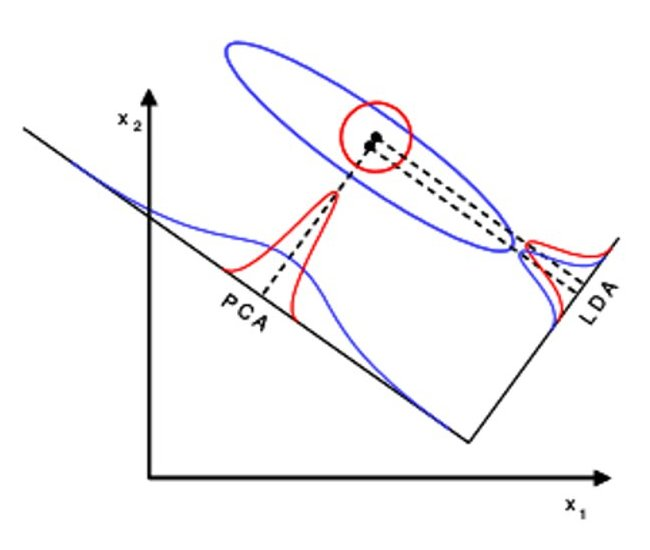
\includegraphics[scale=0.5]{img/limitation_lda}
  \caption{Two classes with similar means and different variances}
  \label{fig:lda-fail}
\end{figure}

Let's call the red class the A class, and the blue one the B. The mean
of A and the mean of B are very close. They are just a slight
translation in one direction, and the LDA will project the data on the
side marked as ``LDA''. And obviously, this is not the good choice.

In the literature, there are several proposition to solve this problem.
The HLDA is one of them.
